\section{Formal Semantics}\label{sec:formal}
\subsection{Grammar}

\marco{Tentative Grammar ClassLessJava}

\begin{figure}[h]
\begin{grammar}
\production{
\e
}{
  \x\mid\MCall\e\m\es\mid\MCall{\C}\m\es\mid\MCall{\C\QM{.super}}\m\es\mid\obj
  }{expressions}\\
\production{
\obj
}{
\QM{new}\ \C\oR\cR\oC\T_1\ \f_1\QM;\ldots\T_k\ \f_k\QM;\
\mh_1\oC\QM{return}\ \e_1\QM{;}\!\cC
\ldots
\mh_n\oC\QM{return}\ \e_n\QM{;}\!\cC
\cC
  }{object creation}\\
\production{
\metaVar{I}
}{
 \ann\ \QM{interface}\ \C_0\ \QM{extends}\ \C_1\ldots\C_k \oC\method_1\ldots\method_n\cC
  }{interface declaration}\\
\production{
\method
}{
 \QM{static}\ \mh\ \oC\QM{return}\ \e\QM{;}\!\cC
\mid
\QM{default}\ \mh\oC\QM{return}\ \e\QM{;}\cC
\mid
\mh\QM{;}
  }{method declaration}\\
\production{
\mh
}{
 \T_0\ \m\ \oR\T_1\ \x_1\ldots\T_n\ \x_n\cR
  }{method header}\\
\production{
\ann
}{
  \mixinAnn|\emptyset
  }{annotations}\\
\end{grammar}
\caption{Grammar of ClassLess Java}
\label{Grammar}
\end{figure}

In Figure~\ref{Grammar} we show the syntax of ClassLess Java.

To be compatible with java, the concrete syntax for an interface declaration with empty supertype list $\C_1\ldots\C_k$ would also omit the \Q@extends@ keyword.

Yanlin and Haoyuan

We need to show 2 things:

1) The dynamic semantics: what's the code that gets generated by a mixin annotation;

2) The type system: what programs to reject; properties: generation of type-safe/checkable code.

\bruno{The implementation is still missing the type system (rejecting some
  programs)!}

\footnote{Future work: updating multiple fields in one method call,
  \texttt{with(T v)}}


\subsection{Typing Rules}
\subsubsection{Expression Typing}

\[
\inferrule{}{\Gamma \vdash x \in \Gamma(x)} \quad \textsc{(T-Var)}
\]

\[
\inferrule{\Gamma \vdash e_0 \in C_0 \\
  \textsf{mtype}(m,C_0) = \overline{D} \to E \\
  \Gamma \vdash \overline{e} \in \overline{C} \\
  \overline{C} <: \overline{D} }
{ \Gamma \vdash e_0.m(\overline{e}) \in E }
\quad \textsc{(T-Invk)}
\]

\[
\inferrule{\textsf{mtype}(m,C) = \overline{D} \to E \\
\Gamma \vdash \overline{e} \in \overline{C} \\
\overline{C} <: \overline{D} \\
\textsf{mmodifier}(m,C) = \textbf{static} }
{\Gamma \vdash C.m(\overline{e}) \in E}
\quad \textsc{(T-StaticInvk)}
\]
\marco{rule tInvk must check is not static?}
\[
\inferrule{\textsf{mtype}(m,C) = \overline{D} \to E \\
\Gamma \vdash \overline{e} \in \overline{C} \\
\overline{C} <: \overline{D} \\\\
\textbf{this}:I \\  I <: C }
{\Gamma \vdash C.\textbf{super}.m(\overline{e}) \in E}
\quad \textsc{(T-SuperInvk)}
\]

\[
\inferrule[(Obj)]{
\forall i\in 1\ldots n\ \Gamma,\Gamma^{\mh_i}\vdash\e_i\in \_\subtype\C^{\mh_i}\\
\forall\mh\in \mhs \mbox{ such that }
\mBody(\m^\mh,\C)=\method;\mh\subtype\mh^\method\\
\forall\m \mbox{ such that }
\mBody(\m,\C)\in\{\mh\QM;,\conflicted\mh\QM;\} \exists \mh_i \in\mhs\mbox{ such that }\mh_i\subtype\mh\\
\Gamma=\Gamma',\f_1{:}\T_1,\ldots,\f_k{:}\T_k,\,\QM{this}{:}\C\\
\mhs=\mh_1\ldots\mh_n
}{
\Gamma' \vdash\QM{new}\ \C\oR\cR\oC\T_1\ \f_1\QM;\ldots\T_k\ \f_k\QM;\
\mh_1\oC\QM{return}\ \e_1\QM{;}\!\cC
\ldots
\mh_n\oC\QM{return}\ \e_n\QM{;}\!\cC
\cC
\in\C
}
\]


\subsubsection{Typechecking of Methods}

\marco{I can not understand those rules, when is t-meth and t-meth body called? when is that you state that all methods in all interfaces must be ok?}
\begin{comment}
\[
\inferrule
{ }
{T_0 \spc m(\overline{T} \spc \overline{x}); \text{ OK IN I} }
\quad \textsc{(T-Meth)}
\]

\[
\inferrule
{\overline{x}:\overline{T} \vdash e:S \\ S <: T_0}
{T_0 \spc m(\overline{T} \spc \overline{x}) \text{ \{ return } e;\} \text{ OK IN
    I} \\\\ \Gamma \vdash \textbf{this}:I }
\quad \textsc{(T-MethBody)}
\]
\end{comment}

\[
\inferrule
{IT(I)=\text{interface } I \text{ extends } \overline{J} \text{\{...\}} \\
\forall i,\text{if \textsf{mtype}}(m,J_i) = \overline(T) \to U_0, \text{then }
T_0 <: U_0 }
{T_0 \spc m(\overline{T} \spc \overline{x}); \text{ OK IN I} }
\quad \textsc{(T-MethExt)}
\]

\[
\inferrule
{\textbf{this}:I, \overline{x}:\overline{T} \vdash e:S \\ S <: T_0 \\
IT(I)=\text{interface } I \text{ extends } \overline{J} \text{\{...\}} \\
\forall i,\text{if \textsf{mtype}}(m,J_i) = \overline(T) \to U_0, \text{then }
T_0 <: U_0 }
{T_0 \spc m(\overline{T} \spc \overline{x}) \text{ \{ return } e;\} \text{ OK IN
    I} }
\quad \textsc{(T-MethBodyExt)}
\]

\subsubsection{Typechecking of Interfaces}
\[ \inferrule
{\textbf{interface } I \textbf{ extends } \overline{J} \{ \overline{M} \} \\\\
 \forall J_i \in \overline{J}, J_i \text{ OK} \\\\
 \forall m \in \overline{M}, \textsf{mbody}(m,I) \neq ERROR \\\\
 \forall J_i \in \overline{J}, \forall m \text{ inside } J_i,
 \textsf{mbody}(m,I) \neq ERROR }
{I \text{ OK}}
\quad \textsc{(T-Intf)}
 \]

Interface $I$ type checks well, if:
\begin{itemize}
\item All its super-interfaces $\overline{J}$ OK.
\item All methods inside interface $I$ are OK.
\item All methods that $I$ is inheriting from super-interfaces are OK.      
\end{itemize}

\subsubsection{Context}
\[ \Gamma :: = \overline{x}:\overline{C} \]

The environment $\Gamma$ is a mapping from variables to types, written
$\overline{x}:\overline{C}$. Typing statement $\Gamma \vdash t:C$ reads ``in the
environment $\Gamma$, term $t$ has type $C$.'' We abbreviate typing statements on
sequences in a simple way, writing $\Gamma \vdash \overline{t}:\overline{C}$ as
shorthand for $\Gamma \vdash t_1:C_1,..., \Gamma \vdash t_n:C_n$.

\subsubsection{Subtyping}

\[ \inferrule{}{T <: T} \]

\[ \inferrule{S <: T \\ T <: U}{S <: U}\]

\[ \inferrule{\emph{ann} \spc \textbf{interface} \spc C_0 \spc \textbf{extends} \spc C_1,...,C_k \{...\}}
{C_0 <: C_1 \\ ... \\ C_0 <: C_k} \]

\subsubsection{Interface Table}
The Interface Table (IT) mapping from types \texttt{T} to interface declarations \texttt{L}. From the
interface table, we can read off the subtype relation between interfaces. The
subtype relation is given by the \textbf{extends} clauses in \texttt{IT}.


\subsection{Auxiliary Definitions}

\begin{comment}
\subsubsection{Auxiliary function: \textsf{mtype}}
- \textsf{mtype(m, C)} : the signature of method m in C.

\[ \inferrule{
  IT(T) = \text{\emph{ann} interface } C \{ \overline{M} \} \\
  E \spc m(\overline{D} \spc \overline{x}) \{ \text{return } e; \} \in M}
{ \textsf{mtype(m,T)} = \overline{D} \to E } \]

\[ \inferrule{
  IT(T) = \text{\emph{ann} interface } C \{ \overline{M} \} \\
  m \notin M}
{ \textsf{mtype(m,T)} = \emptyset } \]

\[ \inferrule{
  IT(T) = \text{\emph{ann} interface } C \text{ extends } C_1,...,C_k \{ \overline{M} \} \\
  E \spc m(\overline{D} \spc \overline{x}) \{ \text{return } e; \} \in M}
{ \textsf{mtype(m,T)} = \overline{D} \to E } \]

\[ \inferrule{
  IT(T) = \text{\emph{ann} interface } C_0 \text{ extends } \overline{C} \{
  \overline{M} \} \\
  m \notin M}
{ \textsf{mtype(m,T)} = \bigcup \textsf{mtype}(m,\overline{D}) } \]
\end{comment}

\subsubsection{Functional notation}
We allows functional notation for set of methods $\methods$, using the method name $\m$ as a key.
That is, we define $\methods(\m)=\method$ iff there is a unique $\method\in\methods$ whose name is $\m$.
For convenience, we define $\methods(\m)=\none$ otherwise.

\subsubsection{Auxiliary function:\mBody}

$\mBody(\m,\C)$ denotes the actual body of method $\m$ that interface $\C$ owns. It can either be defined originally in $\C$ or in its supertypes, and then passed to $\C$ via inheritance.

The body of a method $\m$ contains all the relevant information with respect to that method, like the type of $\m$ as well as the modifier.
We use internally a special modifier $\conflicted$ to denote the case of two methods with conflicting implementation.
%
%\[ \inferrule{
%  IT(C) = \text{\emph{ann} interface } C \{ \overline{M} \} \\
%  m \notin M}
%{ \textsf{mbody}(m,C) = \emptyset } \]
%
%\[ \inferrule{
%  IT(C) = \text{\emph{ann} interface } C \{ \overline{M} \} \\
%  m \in M}
%{ \textsf{mbody}(m,C) = m } \]
%
%\[ \inferrule{
%  IT(C_0) = \text{\emph{ann} interface } C_0 \text{ extends } \overline{C} \{
%  \overline{M} \} \\
%  m \notin M
%  }
%{ \textsf{mbody}(m,C_0) = \textsf{fold}_\textsf{shadow}\cdot\textsf{map}_{\textsf{mbody,}m}\cdot\textsf{subset}(\overline{C}) } \]

\[ \inferrule[(ReviewedRule)]{
  IT(C_0) = \text{\emph{ann} interface } C_0 \text{ extends } \overline{C} \{
  \methods \}
%\\
 % \methods(\m)=\method
%\\
%\Aux{tops}(\overline{C})=\C_1\ldots\C_n
  }
{ \mBody(\m,\C_0) = \override(\methods(\m), %\shadow(\mBody(\m,C_1)\ldots\mBody(\m,C_n))
\shadow(\m,\Aux{tops}(\Cs)))
} \]
\subsubsection{Auxiliary function: $\tops(\Cs), \shadow(\m,\Cs),\override(\method,\method')$}
${}_{}$\\*
\marco{we need to discuss the names tops, shadow and override}

\tops{} leave only the ``needed'' superinterfaces, that is, the ones that are not transitivelly reachable by following another superinterface chain.

\shadow{} choose the most specific version of a method, that is the unique version available, or a conflicted version from a set of possibilities.
We do not model overloading, so it is an error if multiple versions are available with different parameter types.

%The \textsf{shadow} function takes two same methods (with the same name and types of arguments), and return the method which shadows the other during inheritance.
%exmples to motivate our design
%interface A{static String m(){return "A";}}
%interface C extends A{
%	default String dm(){
%		  this.m();//wrong in java
%		  A.m();
%		  C.m();//wrong in java
%		}
%}
%
%
%(1) Static methods are not inherited. Also, if one of $\{body_1,body_2\}$ is null, \textsf{shadow} simply returns the other one. Hence

\yanlin{for \textbf{shadow} conflicted mh;, one missing case is when there are
  two conflicting default methods with same signature?? }

\begin{figure}[tbp]
\centering
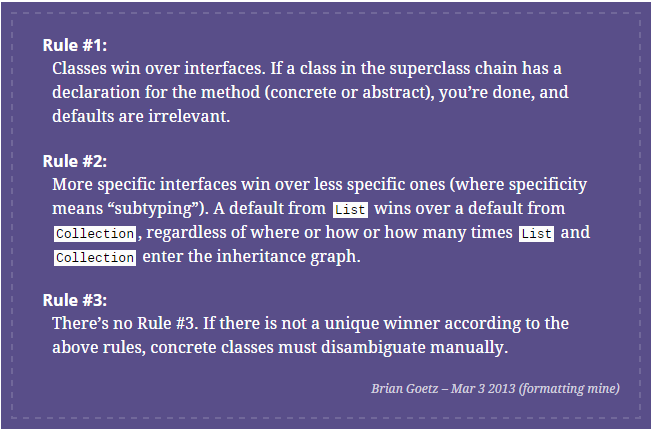
\includegraphics[width=5in]{screenshot.png}
\caption{Screenshot.}\label{screenshot_png}
\end{figure}

\haoyuan{I tried to understand the current algorithm, and did more experiments in eclipse.
Now I borrow some ideas from the current version, and give a new version of the algorithm in text. See below.

(1) I guess the function \textsf{tops} is not necessary. The first step is still
\[\textsf{mbody}(m,C_i)\in\overline{meth}\textrm{ (excluding \textbf{static} methods)}\]

(2) Assume the context is ``interface $C_0$ extends $\overline{C}$ \{$meth'$;...\}''. First handle
\[\textsf{override}(meth',\overline{meth}) \eqno{(*)}\]

(3) If $meth'\ne\none$, $(*)$ returns $meth'$ if
\[\forall meth\in\overline{meth},meth'\subtype meth\]
even if there are conflicts in $\overline{meth}$.

(4) If $meth'=\none$, we need to figure out
\[\textsf{mostSpecific}(\overline{meth})\]
and it should be the one that ``overrides'' all the others in $\overline{meth}$. It means we should not only deal with the return types of methods, but also look into the subtyping relation of interfaces. But for abstract methods, only return types are taken into consideration.
}

\begin{figure}[tbp]
\centering
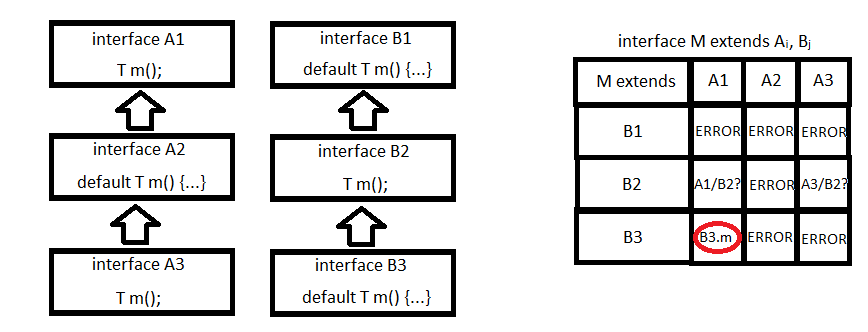
\includegraphics[width=5in]{table.png}
\caption{Table.}\label{table_png}
\end{figure}

\haoyuan{
I found this from the Internet. See Fig.~\ref{screenshot_png}.

An experiment. See Fig.~\ref{table_png}.
}




\begin{equation*}
\begin{array}{ll}
\tops(\Cs)=\{\ \C\in\Cs\ |\ \nexists \C'\in\Cs\setminus\C,\ \C' \subtype \C\ \}
\\
\shadow(\m,\C_1\ldots\C_n)=\shadow(\methods)
& \mBody(\m,\C_i)\in\methods
\\ & \mif\ \mBody(\m,\C)\in\{\mh\QM;,\QM{default}\ \mh\mbox{\Q@\{return \_;\}@}\}
%\\ &\mor\ \mBody(\m,\C)=\mh\QM;
\\

\shadow()=\none\\
\shadow(\method)=\method\\
\shadow(\methods)=\Aux{mostSpecific}(\methods) &\mif\   \methods=\mh_1\QM;\ldots\mh_n\QM;\\
\shadow(\methods)=\conflicted\mh\QM;&\mif\ \Aux{mostSpecific}(\methods))\in\{\mh\QM;,\QM{default}\ \mh\mbox{\Q@\{return \_;\}@}\}\\
\Aux{mostSpecific}(\methods)=\method &
\mif\ \method \in \methods, \forall \method' \in \methods :  \method \subtype
                                       \method', \\
\T\ \m\oR\T_1\x_1\ldots \T_n\x_n\cR \subtype \T' \m\oR\T_1\x_1'\ldots\T_n\x_n'\cR & \mif\ \T\subtype \T'\\

\method \subtype
\QM{default}\ \mh\mbox{\Q@\{return \_;\}@}=
\method\subtype\mh\QM;
\\
\QM{default}\ \mh\mbox{\Q@\{return \_;\}@}\subtype\method=
\mh\QM;\subtype\method
\\
\override(\none,\none)=\none\\
\override(\method,\none)=\method\\

\override(\none,\method)=\method &\mif\ \method\neq \conflicted\ \mh\QM;\\
\override(\method,\method')
=
\override(\method,\mh\QM;) & \method'\in\{\QM{default}\ \mh\mbox{\Q@\{return \_;\}@}, \conflicted\ \mh\QM; \}\\
\override(\method,\mh')
=\method &\mif\ \method\in\{\mh\QM;,\QM{default}\ \mh\mbox{\Q@\{return \_;\}@} \}\\
& \mh\subtype\mh'\\
%\textsf{shadow}(body_1, body_2)=\emptyset & \textsf{if }body_1.\textsf{modifier}=body_2.\textsf{modifier}=\textbf{static}\\
%\textsf{shadow}(body_1, body_2)=body_1 & \textsf{if }body_2=\emptyset\textsf{ or }body_2.\textsf{modifier}=\textbf{static}\\
%\textsf{shadow}(body_1, body_2)=body_2 \hspace{.1in}  & \textsf{if }body_1=\emptyset\textsf{ or }body_1.\textsf{modifier}=\textbf{static}
\end{array}
\end{equation*}

%\text{\yanlin{shouldn't mostSpecific be: $\forall \method' \in \methods : \method \subtype
%  \method'$ ?}}

%(2) If $body_1.\textsf{returnType}=body_2.\textsf{returnType}$, \textsf{shadow} tends to return a default method. If both $body_1$ and $body_2$ are default methods, \textsf{shadow} throws an error.
%\begin{equation*}
%\begin{array}{ll}
%\textsf{shadow}(body_1, body_2)=\textsf{ERROR} & \textsf{if }body_1.\textsf{modifier}=body_2.\textsf{modifier}=\textbf{default}\\
%\textsf{shadow}(body_1, body_2)=body_1 \hspace{.1in} & \textsf{if }body_1.\textsf{modifier}=\textbf{default} \\
%\textsf{shadow}(body_1, body_2)=body_2 \hspace{.1in} & \textsf{if }body_2.\textsf{modifier}=\textbf{default} \\
%\textsf{shadow}(body_1, body_2)=body_1\textsf{ (or }body_2\textsf{)} \hspace{.1in} & \textsf{otherwise}
%\end{array}
%\end{equation*}
%
%(3) If $body_1.\textsf{returnType}<:body_2.\textsf{returnType}$, \textsf{shadow} tends to choose the one with the subtype (namely $body_1$), but only when both methods are abstract, otherwise it gives an error. The other direction $body_2.\textsf{returnType}<:body_1.\textsf{returnType}$ follows the same rule. It also gives an error if there is no subtyping relationship between two return types.
%\begin{equation*}
%\begin{array}{ll}
%\textsf{shadow}(body_1, body_2)=body_1 & \textsf{if }body_1.\textsf{modifier}=body_2.\textsf{modifier}=\emptyset\\
%& \textsf{and }body_1.\textsf{returnType}<:body_2.\textsf{returnType}\\
%\textsf{shadow}(body_1, body_2)=body_2 & \textsf{if }body_1.\textsf{modifier}=body_2.\textsf{modifier}=\emptyset\\
%& \textsf{and }body_2.\textsf{returnType}<:body_1.\textsf{returnType}\\
%\textsf{shadow}(body_1, body_2)=\textsf{ERROR} \hspace{.1in} & \textsf{otherwise}
%\end{array}
%\end{equation*}

%\subsubsection{Auxiliary function: \textsf{replace}}
%
%The \textsf{replace} function takes two same methods (with the same name and types of arguments), and gives the result of the first method overriding the second one.
%
%\begin{equation*}
%\begin{array}{ll}
%\textsf{replace}(body_1, body_2)=body_1 & \textsf{if }body_2=\emptyset\\
%\textsf{replace}(body_1, body_2)=body_2 & \textsf{if }body_1=\emptyset\\
%\textsf{replace}(body_1, body_2)=body_1 & \textsf{if }body_1.\textsf{returnType}<:body_2.\textsf{returnType}\\
%\textsf{replace}(body_1, body_2)=\textsf{ERROR} \hspace{.1in} & \textsf{otherwise}
%\end{array}
%\end{equation*}



\subsubsection{Derived notations}

 Below shows how the functions $mtype$ and $mmodifier$ are derived from $mbody$.

\[ \textsf{mbody}(m,C) = \textit{modifier } E \spc m(\overline{D} \spc \overline{x}) \{ \text{return } e; \} \] \[ \Rightarrow \textsf{mtype}(m,C) = \overline{D} \to E,\ \textsf{mmodifier}(m,C) = \textit{modifier}\]

%\marco{we also need to define a function that gives all the methods of an interface, something line}
%\[
%\Aux{methodsOf}_\C=\{\m|\mBody(\m,\C)=\method\}
%\]
